\documentclass{article}

\usepackage{graphicx}
\usepackage{hyperref} %this should always be the last package

\newcommand{\mytitle}{Multi-thread simulation of a large scale dynamical system}
\let\oldmarginpar\marginpar
\renewcommand{\marginpar}[1]{\oldmarginpar{\raggedright #1}}
\newtheorem{requirement}{Requirement}
\newcommand{\e}{\epsilon}
\newlength{\rulewidth}\setlength{\rulewidth}{0.4pt}
\newcommand{\myrule}{\noindent\rule{\textwidth}{\rulewidth}}
\newcommand{\combvar}{Kg} % TODO: remove
% \texttrademark

\hypersetup{
	pdfauthor={Diego Bellani},
	pdftitle={\mytitle},
	pdfsubject={Bachelor thesis},
	pdfkeywords={bachelor,thesis,programming},
	pdfproducer={LaTeX},
	pdfcreator={pdfLaTeX},
	pdfborder={0 0 0},
	pageanchor=false
}

\title{\mytitle}
\date{2021}
\author{Diego Bellani\thanks{Student}\and Enrico Tronci\thanks{Supervisor}}

\begin{document}

\begin{titlepage}
	\pagenumbering{roman}
	\maketitle

	\begin{abstract}
	(Max one page, da scrivere alla fine)
	\end{abstract}

	\tableofcontents
	\iffalse
	\listoffigures
	\listoftables
	\fi
\end{titlepage}

% TODO: citare il più possibile e fare ricerca sulle varie cose citate
% * devo integrare il vecchio documento in the "Methods" section, mentre lo
%   spiego posso parlare dell'approccio preso per passare da un insieme di
%   equazioni ad un programma funzionante, anche perché è dove la maggior parte
%   del lavoro è andato. Tutte le varie \section possono essere trasformate in
%   \subsection.
% * devo parlare del fatto che ho considerato le istruzioni SIMD, in particolare
%   SLEEF
% * devo parlare del processo di ottimizzazione, come sono partito da
%   un'implemetazione banale e sono arrivato a quella corrente, passando per lo
%   skip delle celle, per la trasformazione del sin + cos e in fine per
%   l'introduzione  di OpenMP
% * devo parlare dello schema, fare il diagramma ER, e parlare della sbrodolata
%   di vincoli in FOL
% * devo dire che un possibile miglioramento del mio codice potrebbe essere
%   quello di mettere N e B in due array separati per velocizzare il look up di
%   N ma nessun miglioramento è stato misurato, quindi neanche la versione bit
%   array è stata provata
% * devo parlare del black book of graphics programming e della sua solizione
% * devo inserire la foto di un tipico incendio per poter introdurre
%   l'assunzione principale, ovvero che le celle in fiamme sono poche
% * devo nicludere delle metriche sul codice e.g. il numero di linee di codice

% ERRORI TROVATI:
% * la probabilità deterministica (si erano scordati di dirci quali termini
%   perturbare)
% * divisioni per zero
% * mancanza di unità di misura
% * funzioni senza definizioni e mal poste (gamma può dare al più tre output per
%   amor del vero)
% * non è stato specificato cosa fare sulle condizioni del bordo

\pagenumbering{arabic}

\section{Introduction}\label{sec:intro}

(da scrivere alla fine) internship report

\subsection{Context}\label{sec:context}
% Short description of context

Firefighting in forests is a complex activity due to the limited availability of
means and resources. Therefore the intervention strategy have to consider the
possible evolution of the fire to make the best use of what is available.

The possible evolution of a fire can be charaterized with a mathematical model
and predictred with a faster-then-real-time simulation of said model. Given this
actions can be taken ahead of time to minimize the damage caused by the fire and
maximazing the fire extinction speed.

\subsection{Motivations}\label{sec:motivations}
% Motivation for what we want to do
% Describe what is missing and instead would be useful to have

This thesis is part of a project called ``Satellite Driven Fire Simulator'',
financed by the region of Lazio, to aid firefighters fight put out forest fires.
To make this possible a software has to be developed that can show the evolution
of ofrest fires ahead of time.

This project is divided in multiple parts:

\begin{enumerate}
\item development of a mathematical model (done by Paola Russo of the Tor
Vergata university);
\item \label{enum:my_work} development of a software to run the mathematcal
model;
\item \label{enum:interaction} development of a user interface for inputung data
to the simulator and showing the results in a human readable fashion;
\item \label{enum:data} gathering the data from the field, this includes geograpnic data from
satellites \cite{cop} and meteorologic data from on field sensors.
\end{enumerate}

This internship report will talk only about item \ref{enum:my_work}

The original implementation was made in Microsoft
Excel\textsuperscript{\textregistered}, which is fine for prototyping but not
suitable for fast large scale simulations. Therefore a better implementation was
needed both for speed and user friendlyness.

The usual tool we used for implementation of mathematical models, Modelica, did
not made the cut beacuse of it's limitation regarding dinamically sized arrays
and the exponential (?) time taken by the optimization algorithm at the
increasing of the size of the simulation grid.

\subsection{Contributions}\label{sec:contrib}
% Describe here your contributions, namely the missing items identified in the
% motivations.

I have implemented from scrath the simulator making sure of its correctness and
performance. The user interface will be implemented by others. To make
collaboration between me and the other party that will implement the user
interface easier i have also created a database schema together with contrains
to keep the data consistent.

Also, by me and my advisor, some corrections have been proposed to the model in
addition to the dimensional analysis made.

\subsection{Related Work}\label{sec:related_work}
% Describe here the state of the art (e.g., algorithms and tools  available). 
% For each paper/tool explain what you do that it is not already available
% (killing).

The simulator was implemented using only relatively standard techniques. So no
particular algorithm worth of notice was used.

The only tool that I tried to use was Modelica that, as said before, was really
meant to implement other kinds of mthematical models, namely continuous ones.
Libraries exists to develop cellular automata models \cite{calib2}, but with
generality comes a lost in performance.

This said Modelica was still a valuable tool for prototyping a small version of
the model before it's real implementation.

\subsection{Outline}\label{sec:outline}
% Give an outline of the thesis structure (one sentence per section)

In the section \ref{sec:background}\dots In the section \ref{sec:methods}\dots
In the section \ref{sec:methods}\dots In the section
\ref{sec:implementation}\dots In the section \ref{sec:experimental_results}\dots
In the section \ref{sec:conclusions}\dots

\section{Background}\label{sec:background}
% Put in this section all the background knowledge needed to understand what you
% did.

The model is based on a cellular automata \cite{gol}.

The provided server has a modern Intel processor and a Linux based operating
system.

To make the best use of the aveilable hardware the simulator was implemented in
C11 using the OpenMP compiler extension.  Because the server used had a Linux
based operating system on it the C standard library and the POSIX interfaces
were used to comunicate with it\footnote{To make it highly portable and
accomodate eventual changes}. OpenMP was chosen as the threading interface,
instead of the C11 one or the POSIX one, because of it's semplicity of use and
beacuse the model was trivially parallelizable.

OpenMP made possible to keep a relatively clean code even in the face of
frequent changes, but still archive reasonable performances. Also it alowed me
to test first for correctness and then performance, with minimal changes.

A SQL database (Postgresql) was chosen to integrate all the different data
sources and to handle the concurrency. But the simulator inputs and outputs CSV
files \cite{csv}, to be more precise a subset of this format was chosen: quoted
numbers are not supported. This format was chosen due to its simplicity and the
simplicity of the data read and written from and to disk. Another important
factor was the wide support that this format has. Extensive use of the
\texttt{ARRAY} data type introuced in SQL:99 to better model the data tha was,
most of the time a big 2D matrix.

\section{Methods}\label{sec:methods}
% Describe here the algorithm design from a math perspective. No code here.

Per descrivere l'evoluzione di un incendio nella foresta il modello si basa su
tre semplici osservazioni

\begin{enumerate}
\item un incendio brucia finché c'è del combustibile,
\item un incendio consuma combustibile nel tempo e
\item un incendio si può spostare in un'area limitrofa.
\end{enumerate}

Dopo aver diviso un'area rettangolare della foresta in $L^* \times W^*$ celle
quadrate, che in seguito ci permetteranno di descrivere con più precisione le
caratteristiche delle varie zone della foresta, capiamo che di ogni cella, in
riga $i$ e colonna $j$, della foresta ci interessano solo due caratteristiche:
la quantità di combustibile in essa ad un certo istante $B_{ij}(t)$ e la
presenza o meno di un incendio in essa ad un certo istante $N_{ij}(t)$, che può
assumere solo due valori 0 per niente incendio e 1 per incendio. Queste due
funzioni rappresenteranno lo \emph{stato} della cella.

Per modellare il concetto di spostamento dell'incendio in aree limitrofe si è
scelto di utilizzare un automa cellulare \cite{gol}.

Un incendio oltre che avere un singolo punto di innesco ne potrebbe avere vari
nel tempo, ad esempio nel caso di incendi dolosi. Per questo non basta una
semplice nozione di stato iniziale ma ci serve un modo per parlare
dell'input esogeno del sistema, che chiameremo $u_{ij}(t)$, che può sempre
assumere solo due valori 0 per niente incendio e 1 per incendio.

Possiamo formalizzare tutto ciò che abbiamo detto finora con queste equazioni

% TODO: capire qual'è la formula per gamma
\begin{eqnarray}
N_{ij}(0) &=& u_{ij}(0)\textrm{,}\\
B_{ij}(0) &=& \gamma_{ij}\textrm{,}\\
N_{ij}(t+1) &=& \cases{\max(V_{ij}(t), u_{ij}(t)), &se $\overbrace{B_{ij}(t) > 0}^\textrm{c'è combustibile}$;\cr
                       0, &altrimenti.}\\
B_{ij}(t+1) &=& \cases{\max(0, B_{ij}(t)-\beta\tau), &se $\underbrace{N_{ij}(t) > 0}_\textrm{c'è incendio}$;\cr
                       B_{ij}(t), &altrimenti.}
\end{eqnarray}

Dove $\gamma_{ij}$ è la quantità iniziale di combustibile in una cella,
$V_{ij}(t)$ è la possibilità che un l'incendio si sposti nella cella corrente da
una delle sue limitrofe (figura \ref{fig:automata}), $\beta$ è la velocità di
consumo del combustibile e $\tau$ e il passo temporale.
% TODO: \beta deve esere calcolata dai dati a disposizione

\begin{figure}
\centering
\setlength{\unitlength}{0.7cm}
\begin{picture}(6,6)
	\newlength{\piccenter}
	\setlength{\piccenter}{3\unitlength}
	% Grid
	\thicklines
	\multiput(0,0)(2,0){4}{\line(0,1){6}} % columns
	\multiput(0,0)(0,2){4}{\line(1,0){6}} % rows

	% Arrays
	\thinlines
	\put(\piccenter,\piccenter){\vector(1,0){2}}
	\put(\piccenter,\piccenter){\vector(0,1){2}}
	\put(\piccenter,\piccenter){\vector(-1,0){2}}
	\put(\piccenter,\piccenter){\vector(0,-1){2}}
	\put(\piccenter,\piccenter){\vector(1,1){2}}
	\put(\piccenter,\piccenter){\vector(-1,1){2}}
	\put(\piccenter,\piccenter){\vector(1,-1){2}}
	\put(\piccenter,\piccenter){\vector(-1,-1){2}}

	% Black square
	\newlength{\side}
	\setlength{\side}{0.8\unitlength}
	\linethickness{\side}
	\newlength{\ypos}
	\setlength{\ypos}{\piccenter}
	\addtolength{\ypos}{-0.5\side}
	\put(\piccenter,\ypos){\line(0,0){\side}}
\end{picture}
\caption{Automa cellulare}
\label{fig:automata}
\end{figure}

Ovviamente il cuore di questo modello è la funzione $V_{ij}(t)$, che può sempre
assumere solo due valori con la stessa semantica di $N_{ij}(t)$ e $u_{ij}(t)$,
essa è definita nel seguente modo

\begin{eqnarray}
            V_{ij}(t) &=& \max\{\,Q_{ij}(\e_1, \e_2, t) \mid (\e_1, \e_2) \in \Gamma\,\}\textrm{,}\\
               \Gamma &=& \{\,(x, y) \mid x, y \in \{-1, 0, 1\}\,\}\textrm{,}\\
Q_{ij}(\e_1, \e_2, t) &=& \cases{1, &se $p_{ij}(\e_1, \e_2, t) N_{i+\e_1j+\e_2}(t) > \theta$;\cr
                                 0, &altrimenti.}\label{eq:probtest}
\end{eqnarray}

Dove $p_{ij}(\e_1, \e_2, t)$ è la probabilità che l'incendio si sposti dalla
cella limitrofa $(i+\e_1, j+\e_2)$ alla cella corrente $(i, j)$ e $\theta$ è la
soglia di propagazione dell'incendio.

\myrule

Sospendiamo ora la nostra discussione del modelo per descrivere meglio i dati a
nostra disposizione, introdotti nel paragrafo \ref{sec:data}.

Il satellite ci mette a disposizione una serie di dati, descritti nella tabella
\ref{tab:geo}, il significato dei valori e definito nell'appendice
\ref{sec:desc}. Questi tuttavia non sono usati così come sono nel modello ma
sono ``rifiniti'' con le seguenti corrispondenze matematiche.

\begin{table}
\centering
\begin{tabular}{|c|l|c|}
	\hline
	\textbf{Simbolo} & \textbf{Nome} & \textbf{Intervallo valori}\\
	\hline
	$G$ & Foreste & 0,1,2,255\\
	$U$ & Urbanizzazione & 0,\ldots,100,255\\
	$W1$ & Water1 & 0,\ldots,4,253,255\\
	$W2$ & \underline{Water2} & 0,1\\ % NOTE: currently unused
	$P$ & Altimetria & 0,\ldots,4380\\
	\hline
\end{tabular}
\caption{Dati geografici per le singole celle.}
\label{tab:geo}
\end{table}

\marginpar{Nel paragrafo \ref{sec:implementation} vengono fatte delle
precisazioni su alcune di queste corrispondenze.}

\begin{equation}\label{eq:height}
H_{ij} = \cases{1 + G_{ij}, &se $0 \leq G_{ij} \leq 2$;\cr
                  0, &se $G_{ij} = 255$.}
\end{equation}

è l'altezza media della vegetazione nella cella,

\begin{equation}\label{eq:inhabitants}
A_{ij} = \cases{U_{ij}/100, &se $0 \leq U_{ij} \leq 100$;\cr
                0, &se $U_{ij} = 255$.}
\end{equation}

è la percentuale di abitatato nella cella,

\begin{equation}\label{eq:water}
W_{ij} = \cases{0, &se $W1_{ij} = 0$;\cr
                1, &se $W1_{ij} = 1$;\cr
                0.75, &se $W1_{ij} = 2$;\cr
                0.75, &se $W1_{ij} = 3$;\cr
                0.5, &se $W1_{ij} = 4$;\cr
                1, &se $W1_{ij} = 253$;\cr
                1, &se $W1_{ij} = 255$.}
\end{equation}

è la percentuale di acqua presente. Questi ultimi tre valori ci servono per
calcolare

\begin{equation}
S_{ij} = H_{ij} \cdot (1-A_{ij}) \cdot (1-W_{ij})\textrm{,}\\
\end{equation}

che è la percentuale di infiammabilità della cella, da notare che $A_{ij}$ la
diminuisce probabilmente perché si considerano come zone abitate quelle col
cemento.

In fine

\begin{equation}
P_{ij} = P_{ij}\textrm{,}
\end{equation}

che  è l'altezza media ed è l'unico valore che non viene cambiato.

% TODO: descrivere il comportamento del vento (gaussiano)
Mentre delle stazioni meteo sul posto ci daranno dati riduardo la velocità e la
direzione del vento\dots TODO: NON È ANCORA CHIARO COME FUNZIONANO.

\begin{eqnarray}
	F_{ij} &=& ??\\
	D_{ij} &=& ??
\end{eqnarray}

Sucessivamente nel modello saranno usate solo $S_{ij}$, $P_{ij}$, $F_{ij}$ e
$D_{ij}$.

\myrule

Ora che sappiamo quali dati abbiamo disposizione, possiamo dare una definizione
della possibilità di trasmisione dell'incendio $p_{ij}(\e_1, \e_2, t)$, della
funzione \ref{eq:probtest}.

\begin{equation}\label{eq:prob}
p_{ij}(\e_1, \e_2, t) = k_0 S_{ij} C_{i+\e_1j+\e_2}(t) d(\e_1, \e_2) f_w f_P\textrm{,}
\end{equation}

% NOTE: $k_0$ è UN parametro o IL parametro?
dove $k_0$ è un parametro di ottimizzazione di soglia e

\begin{equation}\label{eq:combust}
C_{i+\e_1j+\e_2}(t) = \sin\left(\pi\frac{B_{i+\e_1j+\e_2}(t)}{\gamma_{i+\e_1j+\e_2}}\right)\textrm{,}
\end{equation}

è lo stato di combustione della cella. Largomento di $C_{ij}(t)$ può assumere
solo valori tra 0 e $\pi$, quindi avra un grafico come quello in figura
\ref{fig:sin}, overro quando metà del carburante è stato consumato allora
l'incendio avrà la massima potenza.

\begin{figure}
\centering
\setlength{\unitlength}{1cm}
\newlength{\mylength}\setlength{\mylength}{3\unitlength}
\begin{picture}(\mylength,\mylength)(0,0)
	\multiput(.5\mylength,0)(0,.1\mylength){10}{\line(0,1){.05\mylength}}
	\put(0,0){\vector(1,0){\mylength}} % ascissas
	\put(0,0){\vector(0,1){\mylength}} % ordinates

	% Magic numbers from: https://stackoverflow.com/questions/29022438/how-to-approximate-a-half-cosine-curve-with-bezier-paths-in-svg
	\qbezier(0,0)(0.3642\mylength,\mylength)(0.5\mylength,\mylength)
	\qbezier(\mylength,0)(0.6358\mylength,\mylength)(0.5\mylength,\mylength)
\end{picture}
\caption{Grafico $\sin(x)$ tra 0 e $\pi$}
\label{fig:sin}
\end{figure}

\begin{equation}\label{eq:disom}
d(\e_1, \e_2) = \left(1-\frac{1}{2}|\e_1\e_2|\right)\textrm{,}
\end{equation}

è il fattore di fattore di disomogeneità al confine delle celle. Esso può
assumere solo due valori 1 e $1/2$, il primo nelle celle sopra, sotto e ai lati
della cella corrente, il secondo sulle celle diagonali. Ovvero l'incendio si
trasmette la metà da una cella diagonale, come mostrato in figura
\ref{fig:disom}.

\begin{figure} % TODO: fix nummber positioning
\centering
\setlength{\unitlength}{0.7cm}
\begin{picture}(6,6)
	\setlength{\piccenter}{3\unitlength}
	% Grid
	\thicklines
	\multiput(0,0)(2,0){4}{\line(0,1){6}} % columns
	\multiput(0,0)(0,2){4}{\line(1,0){6}} % rows

	\put(1,5){1/2}
	\put(3,5){1}
	\put(5,5){1/2}
	\put(1,3){1}
	\put(5,3){1}
	\put(1,1){1/2}
	\put(3,1){1}
	\put(5,1){1/2}

	% Black square
	\setlength{\side}{0.8\unitlength}
	\linethickness{\side}
	\setlength{\ypos}{\piccenter}
	\addtolength{\ypos}{-0.5\side}
	\put(\piccenter,\ypos){\line(0,0){\side}}
\end{picture}
\caption{Disomogeneità al confine tra le celle.}
\label{fig:disom}
\end{figure}

\marginpar{Dare una spegazione intuitiva della semantica delle funzioni
\ref{eq:wind} e \ref{eq:slope}}

\begin{equation}\label{eq:wind}
f_w = \exp\left(k_1 F_{i+\e_1j+\e_2}\frac{\begin{array}{c}\e_1\cos(D_{i+\e_1j+\e_2})\\
      +\\\e_2\sin(D_{i+\e_1j+\e_2})\end{array}}{\sqrt{\e_1^2 + \e_2^2}}\right)
\end{equation}

è il contributo dato dal vento, dove $k_1$ è il parametro di ottimizzazione di
questo contributo, in fine

\begin{equation}\label{eq:slope}
f_P = \exp\left(k_2\arctan\left(\frac{P_{ij}-P_{i+\e_1j+\e_2}}{L}\right)\right)
\end{equation}

è il contributo dato da il dislivello tra le due celle, dove $k_2$ è il
parametro di ottimizzazione di questo contributo.

Tutti i parametri globali del modello e delle singole celle sono stati messi
nelle tabelle riassuntive \ref{tab:globals} e \ref{tab:params}.

\begin{table}
\centering
\begin{tabular}{|c|l|c|}
	\hline
	\textbf{Simbolo} & \textbf{Nome} & \textbf{Unità di Misura}\\
	\hline
	$\tau$ & passo temporale & secondi\\
	$L$ & lato della singola cella & metri\\
	$L^*$ & lunghezza area monitorata & metri\textsuperscript{2}\\
	$W^*$ & ampiezza area monitorata & metri\textsuperscript{2}\\
	$\beta$ & consumo combustibile & \combvar/secondo\\
	$\theta$ & probailità propagazione & adimensionale\\
	$k_0$ & ottimizzazione soglia & adimensionale\\
	$k_1$ & ottimizzazione vento & adimensionale\\
	$k_2$ & ottimizzazione pendenza & adimensionale\\
	\hline
\end{tabular}
\caption{Parametri globali del modello.}
\label{tab:globals}
\end{table}

\begin{table}
\centering
\begin{tabular}{|c|l|c|}
	\hline
	\textbf{Simbolo} & \textbf{Nome} & \textbf{Unità di Misura}\\
	\hline
	$H$ & altezza media della vegetazione & metri\\
	$A$ & percentuale abitazione & adimensionale\\
	$W$ & percentuale acqua presente & adimensionale\\
	% NOTE: a quanto pare \gamma è una costante
	$\gamma$ & quantità di combustibile & \combvar\\
	$S$ & percentuale infiammabilità & adimensionale\\
	$P$ & altitudine media & metri\\
	$D$ & direzione del vento & radianti\\
	$F$ & velocità del vento & metri/secondo\\
	\hline
\end{tabular}
\caption{Parametri delle singole celle.}
\label{tab:params}
\end{table}

The implementation requirements were derived by the documents describing the
mathematical model and the ``Satellite Driven Fire Simulator'' project itself.
Let's start with the first already stated in section \ref{sec:context}

\begin{requirement}\label{thm:faster}
To be able to predict the events the simulation needs to run
faster-then-real-time.
\end{requirement}

And there is also a second requirement already stated in point
\ref{enum:interaction} of the enumeration in section \ref{sec:motivations}

\begin{requirement}\label{thm:used}
The simulator have to be utilized by other programs.
\end{requirement}

In the point \ref{enum:data} of the enumeration in section \ref{sec:motivations}
geographic and meteorological data are mentioned, let's look at those in more
detail.

% TODO: scrivere lo schema in FOL e l'algoritmo in matematica (i.e. il modello)

\section{Implementation}\label{sec:implementation}
% describe here how you implemented the functionalities described in the methods
% section.
% Use pseudo code or diagrams.

The simulator has a relatively simple architecture, upon initialization all the
necessary data is read, validated and transformed for use in the simulation.
Also all the memory needed is allocated, to avoid costly calls to
\texttt{malloc(3)} during the simulation, to do this a double buffer technique
has been used.

% TODO: tell thad for input validation meta-programing has been used

To be able to gracefully halt the simulation before its natural halting
condition (i.e. reaching the event horizon or not transmitting anymore fire) a
global variable is used that is cheked at the end of every iteration of the
simulation. This variable is changed only by a signal handler that should be
triggered only if a great change in the input parameters occurs.

C is a notoriously (TODO insert citation) error prone language to program in,
this includes it's integer (and float) conversion, manual memory allocation,
undefined behavior and pointher arithmetic. But tools can help a lot in
producing good quality software. In particular gcc and clang source sanitizers.
Together with compiler warnings a lot of bugs were cought at compilation time or
in the first execution done for testing after compilation.

Another tecniqued that helped was the use of assertions throught the code to
check invariants, pre-conditions and post-conditions in the various functions
and loops.

At last a tiny feature of OpenMP helped to avoid various bugs namely
\texttt{default(none)} as shown in figure \ref{fig:pragma}. This alowed me to
have precise controll about which variables are shared and which are private, to
avoid race conditions. The actual OpenMP default is \texttt{default(shared)}
that is far too error prone.

\begin{figure}
\centering
\footnotesize
\verb+#pragma omp parallel for collapse(2) default(none) firstprivate(rng_state)+
\verb+shared(s,Gamma,d,sqrt,funcs) reduction(|: has_transmitted_fire)+
\caption{OpenMP \texttt{pragma} used}
\label{fig:pragma}
\end{figure}

\begin{figure}
% https://www.copernicus.eu/en/copernicus-ems-rapid-mapping-activated-forest-fires-central-sweden
\centering
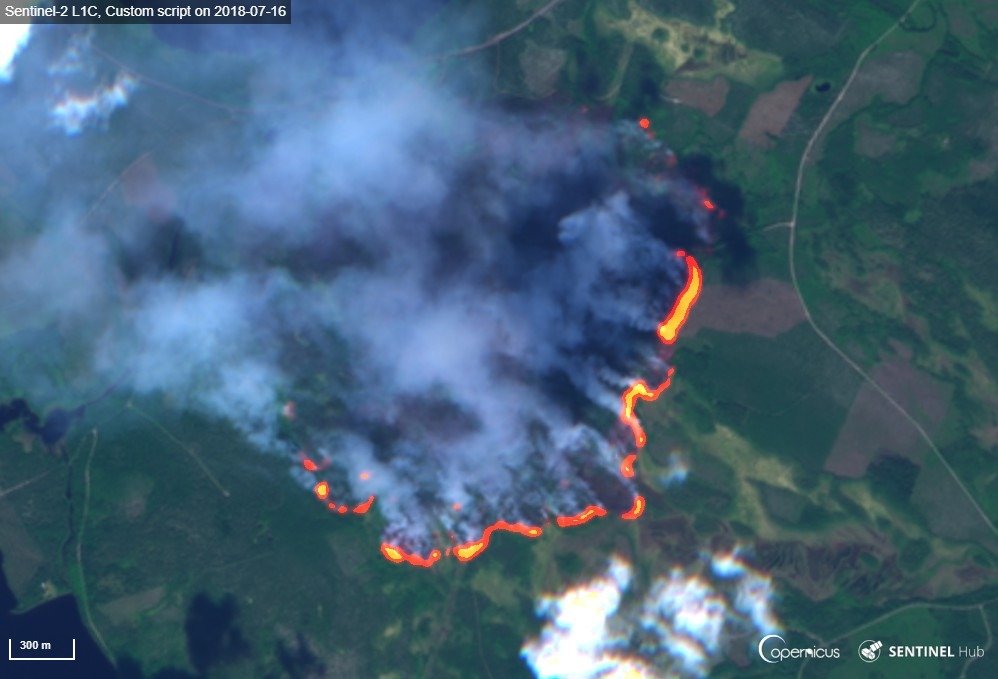
\includegraphics[scale=0.2]{fire.jpg}
\caption{Tipical forest fire.}
\label{fig:fire}
\end{figure}

\begin{table}
\centering
\begin{tabular}{c c | c | c}
$\epsilon_1$ & $\epsilon_2$ & original equation & simplified equation\\
\hline
-1 & 1 & $-\cos(\alpha)+\sin(\alpha)$ & $-\sqrt{2}\sin(\frac{\pi}{4}-\alpha)$\\
0 & 1 & $\sin(\alpha)$ & $\sin(\alpha)$\\
1 & 1 & $\cos(\alpha) + \sin(\alpha)$ & $-\sqrt{2}\sin(\alpha+\frac{\pi}{4})$\\
-1 & 0 & $-\cos(\alpha)$ & $-\sin(\frac{\pi}{2}-\alpha)$\\
1 & 0 & $\cos(\alpha)$ & $\sin(\frac{\pi}{2}-\alpha)$\\
-1 & -1 & $-\cos(\alpha)-\sin(\alpha)$ & $-\sqrt{2}\sin(\alpha+\frac{\pi}{4})$\\
0 & -1 & $-\sin(\alpha)$ & $-\sin(\alpha)$\\
1 & -1 & $\cos(\alpha) + \sin(\alpha)$ & $\sqrt{2}\sin(\frac{\pi}{4}-\alpha)$\\
\end{tabular}
\caption{Simplifications}
\label{tab:simplifications}
\end{table}

\section{Experimental Results}\label{sec:experimental_results}

% describe the experimental results

\subsection{Goals}\label{sec:goals}
% describe here the objectives of the experimental activity;

The experimental activty had the objective of showing performance?? And
correctness udring the operation??

\subsection{Setting}\label{sec:setting}
% describe experimental setting: hardware used, software used, data used, etc...

Mac OS, Instruments.app, \texttt{time(1)}, compiler sanitizers, assert

The software was compiled and tested both on Mac OS and Linux (both real
hardware and virtual machine).

\subsection{Correctness}\label{sec:correctness}

Other than by manual testing the software is ``correct by inspection''
The software has be shown correct after extensive user testing, together with
debugging code (i.e. assertions) enabled and sanitizers.

\subsection{Computational Performance}\label{sec:computational_performance}
% (CPU time and RAM); bytes/sec

Here I can show the difference between parrallel not parallel code.

\section{Conclusions}\label{sec:conclusions}
% Sum up what you did and outline some possible future developments.

Future improvements could be made by abstracting the simualtion code in a
library and make in callable from various languages (e.g. Java, Python etc\dots)
and make integration even easier. Also the core assumption for it's performance
is that the number of cell's on fire is tiny with respect to the others.
Alternative implementations could be given for the opposite scenario. Or the
current one could be re-architected as described in the section about game of
life in the graphics programing black book.

If those techniques turned out usefull they could be abstracted to a library of
general cellular automata based models simulation.

Also in the code the error handling and the logging is a bit messy and could
definately be improved.

\bibliographystyle{plain}
\bibliography{document}

\end{document}
